\documentclass{standalone}
\usepackage{pgf,tikz}
\begin{document}
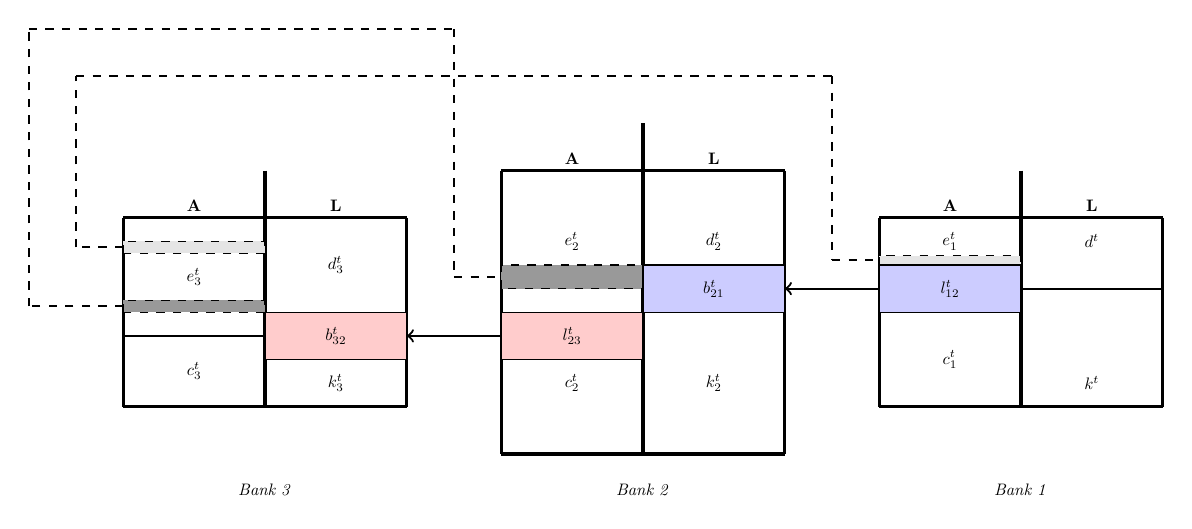
\begin{tikzpicture}[scale=0.6, every node/.style={scale=0.6}]

%%%%%%%%%%%%%%%%%%%%%%%%%%%%%%%%%%%%%%%%%%%%%%%%%%%%%%%%%%%%%%%%
% Downstream periphery
%%%%%%%%%%%%%%%%%%%%%%%%%%%%%%%%%%%%%%%%%%%%%%%%%%%%%%%%%%%%%%%%

% Border and preliminaries
\draw [very thick] (0,5) to (6,5);
\draw [very thick] (6,5) to (6, 1);
\draw [very thick] (6, 1) to (0, 1);
\draw [very thick] (0, 1) to (0, 5);

\draw [very thick] (3, 6) to (3, 1);
    \node [above] at (1.5,5) {\textbf{A}};
    \node [above] at (4.5,5) {\textbf{L}};
    

    
% Initial balance sheet  
%Assets
\node at (1.5, 3.75) {$e_{3}^{t}$};
	\draw [fill=gray!80,dashed] (0,3) rectangle (3,3.25);
	\draw [fill=gray!20,dashed] (0,4.25) rectangle (3,4.5);
 
\node at (1.5,1.75) {$c_{3}^{t}$};
	\draw [thick] (0,2.5) to (3,2.5);

%Liabilities
\node at (4.5,4) {$d_{3}^{t}$};

\draw [fill=red!20] (3,2) rectangle (6,3);

\node  at (4.5,2.5) {$b_{32}^{t}$};
   
\node at (4.5, 1.5) {$k_{3}^{t}$};

%label
\node [above] at (3,-1) {\textit{Bank 3}};

%%%%%%%%%%%%%%%%%%%%%%%%%%%%%%%%%%%%%%%%%%%%%%%%%%%%%%%%%%%%%%%%
% Core
%%%%%%%%%%%%%%%%%%%%%%%%%%%%%%%%%%%%%%%%%%%%%%%%%%%%%%%%%%%%%%%%

% Border and preliminaries
\draw [very thick] (8, 6) to (14, 6);
\draw [very thick] (14, 6) to (14, 0);
\draw [very thick] (14, 0) to (8, 0);
\draw [very thick] (8, 0) to (8, 6);

\draw [very thick] (11, 7) to (11, 0);
    \node [above] at (9.5, 6) {\textbf{A}};
    \node [above] at (12.5, 6) {\textbf{L}};
    
% Initial balance sheet  
%Assets
\node at (9.5,4.5) {$e_{2}^{t}$};
	\draw [fill=gray!80,dashed] (8,3.5) rectangle (11,4);

\draw [fill=red!20] (8,2) rectangle (11,3);
    \node  at (9.5,2.5) {$l_{23}^{t}$};

\node at (9.5,1.5) {$c_{2}^{t}$};

%Liabilities
\node at (12.5, 4.5) {$d_{2}^{t}$};

\draw [fill=blue!20] (11,3) rectangle (14,4);
    \node  at (12.5,3.5) {$b_{21}^{t}$};
    
\node at (12.5, 1.5) {$k_{2}^{t}$};

% label
\node [above] at (11,-1) {\textit{Bank 2}};


%%%%%%%%%%%%%%%%%%%%%%%%%%%%%%%%%%%%%%%%%%%%%%%%%%%%%%%%%%%%%%%%
% Upstream periphery
%%%%%%%%%%%%%%%%%%%%%%%%%%%%%%%%%%%%%%%%%%%%%%%%%%%%%%%%%%%%%%%%

% Border and preliminaries
\draw [very thick] (16,5) to (22,5);
\draw [very thick] (22,5) to (22,1);
\draw [very thick] (22,1) to (16,1);
\draw [very thick] (16,1) to (16,5);

\draw [very thick] (19, 6) to (19, 1);
    \node [above] at (17.5,5) {\textbf{A}};
    \node [above] at (20.5,5) {\textbf{L}};
    
% Initial balance sheet  
%Assets
\node at (17.5,4.5) {$e_{1}^{t}$};
	\draw [fill=gray!20,dashed] (16,4) rectangle (19,4.2);

\draw [fill=blue!20] (16,3) rectangle (19,4);
    \node  at (17.5,3.5) {$l_{12}^{t}$};
    
    \node at (17.5, 2) {$c_{1}^{t}$};
%Liabilities
\node at (20.5, 4.5) {$d^{t}$};
    \draw [thick] (19,3.5) to (22,3.5);
\node at (20.5, 1.5) {$k^{t}$};

% label
\node [above] at (19,-1) {\textit{Bank 1}};

%%%%%%%%%%%%%%%%%%%%%%%%%%%%%%%%%%%%%%%%%%%%%%%%%%%%%%%%%%%%%%%%
% Edges
%%%%%%%%%%%%%%%%%%%%%%%%%%%%%%%%%%%%%%%%%%%%%%%%%%%%%%%%%%%%%%%%

% Interbank
\draw[thick,->] (8,2.5) to (6,2.5); %23
\draw[thick,->] (16,3.5) to (14,3.5); %12

% Overlapping portfolio
% 32 overlap
\draw[thick,dashed]  (0,3.125) to (-2,3.125);
\draw[thick,dashed]  (-2,3.125) to (-2,9);
\draw[thick,dashed]  (-2,9) to (7,9);
\draw[thick,dashed]  (7,9) to (7,3.75);
\draw[thick,dashed]  (7,3.75) to (8,3.75);

% 31 overlap

\draw[thick,dashed]  (0,4.375) to (-1,4.375);
\draw[thick,dashed]  (-1,4.375) to (-1,8);
\draw[thick,dashed]  (-1,8) to (15,8);
\draw[thick,dashed]  (15,8) to (15,4.1);
\draw[thick,dashed]  (15,4.1) to (16,4.1);
\end{tikzpicture}
\end{document}
